\chapter{Evaluierung}\label{chp:evaluierung}
Um die Qualität der Vorhersagen zu bewerten, werden nun die tatsächlichen Schlusskurse mit den vorhergesagten Schlusskursen der Aktien von Amazon verglichen. Die vorhergesagten Schlusskurse beziehen sich auf den Zeitraum vom 6. Dezember bis zum 23. Dezember 2016.

\begin{table}
    \begin{center}
        \begin{tabular}{||c c c c||} 
            \hline
            Datum & \parbox[c]{3.5cm}{\textbf{Tatsächlicher Schlusskurs in \$}} & \parbox[c]{3.5cm}{\textbf{Vorhergesagter Schlusskurs in \$}} & \parbox[c]{3.5cm}{\textbf{Quadratische Abweichung}}\\ [0.5ex] 
        \hline\hline
        06.12.2016 & 764.72 & 771.09 & 40.58 \\ 
    \hline
    07.12.2016 & 770.42 & 776.11 & 32.38 \\
    \hline
    08.12.2016 & 767.33 & 774.92 & 57.61 \\
    \hline
    09.12.2016 & 768.66 & 775.35 & 44.76 \\
    \hline
    12.12.2016 & 760.12 & 776.68 & 274.23 \\ 
    \hline
    13.12.2016 & 774.34 & 768.52 & 33.87 \\
    \hline
    14.12.2016 & 768.82 & 764.50 & 18.66 \\
    \hline
    15.12.2016 & 761.00 & 773.14 & 147.38 \\
    \hline
    16.12.2016 & 757.77 & 778.07 & 412.09 \\
    \hline
    19.12.2016 & 766.00 & 769.03 & 9.18 \\
    \hline
    20.12.2016 & 771.22 & 778.54 & 53.58 \\
    \hline
    21.12.2016 & 770.60 & 780.01 & 88.55 \\
    \hline
    22.12.2016 & 766.34 & 773.54 & 51.84 \\
    \hline
    23.12.2016 & 760.59 & 760.42 & 0.03 \\[1ex]
\end{tabular}
\caption{Vergleich tatsächlicher und vorhergesagter Schlusskurse der Aktie von Amazon}
\label{tab:evaluierung}
\end{center}
\end{table}


Für die tatsächlichen und durch das ML-Modell vorhergesagten Schlusskurse von Amazon in diesem Zeitraum ergeben sich die in \cref{tab:evaluierung} abgebildeten Werte.
Diese zeigt auf, dass sich die durch das ML-Modell vorhergesagten Aktienkurse teilweise im Bereich der tatsächlichen Schlusskurse befindet, die Abweichungen von der Realität einiger Vorhersagen jedoch sehr hoch sind. Außerdem werden in diesem Modell nicht Einflüsse beachtet, die den Verlauf einer Aktie stark beeinflussen könnten. Zu solchen Einflüssen zählen beispielsweise das Erhalten eines umfangreichen Kundenauftrags, Prognosen, die einen Gewinnrückgang erwarten oder steigende Zinsen an den Kapitalmärkten. \cref{fig:chart} zeigt die grafische Darstellung der Schlusskurse im Zeitraum vom 06.12.2016 bis zum 23.12.2016.

\begin{figure}[H]
    \centering
    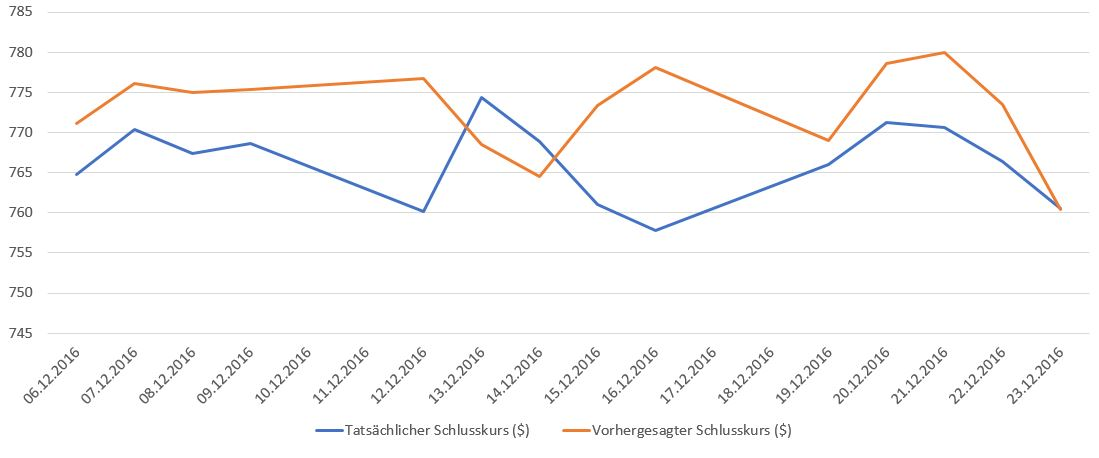
\includegraphics[scale=0.65]{images/Chart.jpg}
    \caption{Tägliche tatsächliche und vorhergesagte Schlusskurse von Amazon}
    \label{fig:chart}
\end{figure}

Eine weitere Methode, um die Qualität der Vorhersagen zu beurteilen ist die Berechnung des Errors der mittleren quadratischen Abweichung (engl. mean squared error). Dafür werden die Abweichungen zwischen den tatsächlichen und den vorhergesagten Schlusskursen quadriert und zum Schluss durch die Anzahl der Vorhersagen geteilt. Für den Error ergibt sich folgender Wert:

\begin{align*}
    MSE &= \frac{1264.74}{14} \\
    MSE &= 90.34
\end{align*}

Somit ergibt sich eine durchschnittliche Abweichung von 90.34, was für einen durchschnittlichen Kurs von etwa 766.28\$ sehr hoch ist. Jedoch sollte auch beachtet werden, dass höhere Abweichungen, wie zum Beispiel am 16.12.2016, auch zu einem höheren durchschnittlichen Fehler führen.

Ferner kann ebenfalls festgestellt werden, dass sich der vorhergesagte Kurs entgegengesetzt zum tatsächlichen Kurs bewegt. So steigt der Kurs des ML-Modells beispielsweise im Zeitraum vom 14. bis 16.12.2016, während in diesem Zeitraum der tatsächliche Kurs fällt. 


Da die Trainingsdaten aus den Jahren 2010 bis 2016 stammen, ist es nicht möglich, mit diesem Modell den morgigen Kurs einer Aktie vorherzusagen. Dazu müssten Trainingsdaten verwendet werden, die nur wenige Monate in der Vergangenheit liegen. Da der Datensatz, der in diesem Projekt verwendet wurde, jedoch nur Informationen bis Ende 2016 beinhaltet, können damit auch nur Vorhersagen in diesem Zeitraum getroffen werden.

Abschließend lässt sich zusammenfassen, dass Aktienkurse durchaus von einem ML-Modell vorhergesagt werden können. Jedoch sollten dabei weitaus mehr Faktoren in das Trainieren des Modells einfließen. Zu solchen Faktoren gehören beispielsweise Prognosen von Banken oder Vermögensverwaltern, Prognosen, die sich positiv oder negativ auf den Aktienkurs auswirken oder ob sich das Unternehmen mitten in einer Krise, wie zum Beispiel der Coronapandemie, befindet. Somit lässt sich sagen, dass der Verlauf einer Aktie nicht nur von mathematischen und statistischen Faktoren abhängt, sondern auch durch psychologische oder extern Rahmenbedingungen beeinflusst werden kann.